\documentclass[11pt]{article}
\usepackage{neurips_2026}

% Additional packages
\usepackage{tikz}
\usetikzlibrary{shapes,arrows.meta,positioning,fit,calc}
\usepackage{algorithm}
\usepackage{algorithmic}
\usepackage{tabularx}
\usepackage{adjustbox}
\usepackage{pifont}
\usepackage{soul}

% Custom commands
\newcommand{\msqa}{\textsc{MSQA-Bench}}
\newcommand{\todo}[1]{\textcolor{red}{\textbf{[TODO: #1]}}}
\newcommand{\placeholder}[1]{\textcolor{blue}{\textbf{#1}}}
\newcommand{\cmark}{\ding{51}}
\newcommand{\xmark}{\ding{55}}

\title{MSQA-Bench: A Large-Scale Question Answering Benchmark \\for Mass Spectrometry Literature}

\author{
  Anonymous Author(s) \\
  \texttt{anonymous@institution.edu}
}

\date{}

\begin{document}

\maketitle

%=============================================================================
% ABSTRACT
%=============================================================================
\begin{abstract}
Mass spectrometry (MS) is a cornerstone analytical technique in proteomics, metabolomics, clinical diagnostics, and environmental science, yet no standardized benchmark exists for evaluating AI-driven question answering (QA) over MS literature.
We introduce \msqa{}, a large-scale QA benchmark constructed from approximately 40,000 peer-reviewed mass spectrometry publications, comprising over 1.2 million question--answer pairs spanning seven question types: factual, method, definition, comparison, numeric, causal, and unknown.
Our automated pipeline extracts text from PDFs, generates QA pairs using a 14B-parameter instruction-tuned language model, and applies multi-stage quality filtering including MinHash deduplication and weighted quality scoring.
We establish comprehensive baselines across two tasks---passage retrieval and closed-book QA---using five fine-tuned embedding models and five QLoRA-adapted large language models.
Fine-tuned embeddings improve Recall@10 by \placeholder{XX}\% over base models, while domain-adapted LLMs achieve \placeholder{XX}\% higher token-level F1 on MS-specific questions.
\msqa{} is released with deterministic document-level splits, quality metadata, and a public-safe export format to facilitate reproducible research in scientific QA.
\end{abstract}

%=============================================================================
% 1. INTRODUCTION
%=============================================================================
\section{Introduction}
\label{sec:introduction}

Mass spectrometry (MS) underpins a vast array of scientific disciplines---from shotgun proteomics and untargeted metabolomics to clinical toxicology and food safety testing. The body of MS literature has grown exponentially, with tens of thousands of papers published annually across journals such as \textit{Analytical Chemistry}, \textit{Journal of the American Society for Mass Spectrometry}, and \textit{Proteomics}. Researchers and practitioners routinely need to query this literature for experimental protocols, instrument parameters, data analysis methods, and comparative results---tasks that are natural candidates for automated QA systems.

Despite significant progress in scientific NLP---including benchmarks for biomedical QA (PubMedQA~\citep{jin2019pubmedqa}, BioASQ~\citep{tsatsaronis2015overview}), chemistry (ChemProt~\citep{taboureau2011chemprot}), and general scientific reasoning (SciQ~\citep{welbl2017crowdsourcing}, SciFact~\citep{wadden2020fact})---no benchmark specifically targets mass spectrometry. This gap is significant because MS literature contains highly specialized vocabulary (e.g., \textit{collision-induced dissociation}, \textit{selected reaction monitoring}, \textit{electrospray ionization}), domain-specific reasoning about instrument configurations and analytical workflows, and quantitative relationships between experimental parameters and outcomes.

General-purpose large language models (LLMs) often struggle with such domain-specific content, producing plausible but factually incorrect answers---a problem exacerbated in high-stakes scientific contexts where hallucinated instrument settings or incorrect method parameters could lead to failed experiments or erroneous conclusions.

In this work, we present \msqa{}, a comprehensive QA benchmark designed to evaluate and advance AI systems for mass spectrometry literature understanding. Our contributions are:

\begin{enumerate}[leftmargin=*,itemsep=2pt]
    \item \textbf{A large-scale domain-specific dataset}: Over 1.2 million QA pairs derived from $\sim$40,000 mass spectrometry publications, with quality filtering, deduplication, and classification into seven question types.

    \item \textbf{An automated, reproducible construction pipeline}: An end-to-end pipeline from raw PDFs to benchmark-ready records, including multi-strategy text extraction, LLM-based QA generation, MinHash deduplication, and deterministic document-level splitting.

    \item \textbf{Comprehensive retrieval and generation baselines}: Evaluation of BM25, five base embedding models, five fine-tuned embedding models, and five QLoRA-adapted LLMs across retrieval and closed-book QA tasks.
\end{enumerate}

%=============================================================================
% 2. RELATED WORK
%=============================================================================
\section{Related Work}
\label{sec:related_work}

\paragraph{Scientific QA Benchmarks.}
The NLP community has developed several benchmarks for scientific question answering. PubMedQA~\citep{jin2019pubmedqa} targets yes/no/maybe questions from PubMed abstracts. BioASQ~\citep{tsatsaronis2015overview} provides a biomedical semantic indexing and QA challenge with annually updated datasets. SciQ~\citep{welbl2017crowdsourcing} offers multiple-choice science exam questions, while SciFact~\citep{wadden2020fact} focuses on scientific claim verification. MMLU~\citep{hendrycks2021measuring} includes science sections but at a broad, exam-level granularity. ChemProt~\citep{taboureau2011chemprot} addresses chemical--protein interactions but is limited to relation extraction rather than open-domain QA.

None of these benchmarks specifically address mass spectrometry---a domain with unique vocabulary, complex analytical workflows, and instrument-specific reasoning. \msqa{} fills this gap with a large-scale, multi-type QA benchmark tailored to MS literature.

\paragraph{Domain-Adaptive Language Models.}
Pre-training or fine-tuning language models on domain-specific corpora has proven effective for scientific NLP. BioBERT~\citep{lee2020biobert} and PubMedBERT~\citep{gu2021domain} demonstrated gains on biomedical tasks through continued pre-training on PubMed abstracts. SciBERT~\citep{beltagy2019scibert} extended this to broader scientific text. For generative models, BioGPT~\citep{luo2022biogpt} showed that domain-specific pre-training improves biomedical text generation. More recently, parameter-efficient methods such as QLoRA~\citep{dettmers2024qlora} have enabled fine-tuning of large models on domain data using consumer-grade GPUs.

We extend this line of work by fine-tuning both embedding models (for retrieval) and instruction-tuned LLMs (for generation) specifically on mass spectrometry QA data, demonstrating the value of domain adaptation for specialized scientific QA.

\paragraph{Synthetic QA Generation.}
Using LLMs to generate training data has become increasingly common. \citet{alberti2019synthetic} showed that synthetic QA pairs from BERT improve reading comprehension. More recently, instruction-tuned models have been used to generate high-quality QA pairs at scale~\citep{wang2023self}. We use Qwen2.5-14B-Instruct-AWQ~\citep{qwen2025qwen25} served via vLLM~\citep{kwon2023efficient} to generate diverse QA pairs from MS paper paragraphs, applying multi-stage quality filtering to ensure benchmark quality.

%=============================================================================
% 3. DATASET CONSTRUCTION
%=============================================================================
\section{MSQA-Bench: Dataset Construction}
\label{sec:dataset}

Figure~\ref{fig:pipeline} illustrates our end-to-end pipeline from raw PDFs to benchmark-ready QA records. We describe each stage below.

\begin{figure}[t]
\centering
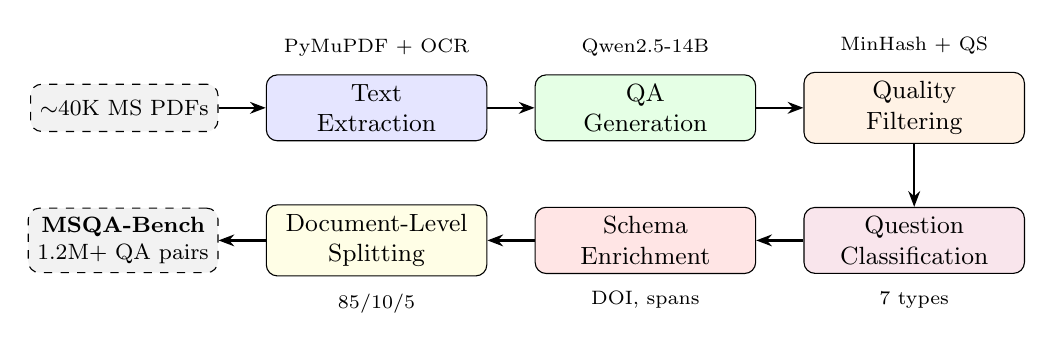
\begin{tikzpicture}[
    node distance=0.6cm,
    box/.style={rectangle, draw, rounded corners, minimum width=2.8cm, minimum height=0.7cm, align=center, font=\small},
    arrow/.style={-{Stealth[length=2mm]}, thick},
    data/.style={rectangle, draw, dashed, rounded corners, minimum width=2.2cm, minimum height=0.6cm, align=center, font=\footnotesize, fill=gray!10}
]
    % Pipeline stages
    \node[data] (pdfs) {$\sim$40K MS PDFs};
    \node[box, right=of pdfs, fill=blue!10] (extract) {Text\\Extraction};
    \node[box, right=of extract, fill=green!10] (qagen) {QA\\Generation};
    \node[box, right=of qagen, fill=orange!10] (filter) {Quality\\Filtering};
    \node[box, below=0.8cm of filter, fill=purple!10] (classify) {Question\\Classification};
    \node[box, left=of classify, fill=red!10] (enrich) {Schema\\Enrichment};
    \node[box, left=of enrich, fill=yellow!10] (split) {Document-Level\\Splitting};
    \node[data, left=of split] (bench) {\textbf{MSQA-Bench}\\1.2M+ QA pairs};

    % Arrows
    \draw[arrow] (pdfs) -- (extract);
    \draw[arrow] (extract) -- (qagen);
    \draw[arrow] (qagen) -- (filter);
    \draw[arrow] (filter) -- (classify);
    \draw[arrow] (classify) -- (enrich);
    \draw[arrow] (enrich) -- (split);
    \draw[arrow] (split) -- (bench);

    % Annotations
    \node[font=\scriptsize, above=0.1cm of extract] {PyMuPDF + OCR};
    \node[font=\scriptsize, above=0.1cm of qagen] {Qwen2.5-14B};
    \node[font=\scriptsize, above=0.1cm of filter] {MinHash + QS};
    \node[font=\scriptsize, below=0.1cm of classify] {7 types};
    \node[font=\scriptsize, below=0.1cm of enrich] {DOI, spans};
    \node[font=\scriptsize, below=0.1cm of split] {85/10/5};
\end{tikzpicture}
\caption{The \msqa{} construction pipeline. Raw mass spectrometry PDFs undergo text extraction, LLM-based QA generation, quality filtering with MinHash deduplication, question type classification, schema enrichment with metadata and evidence spans, and deterministic document-level splitting.}
\label{fig:pipeline}
\end{figure}

\subsection{Source Corpus}
\label{sec:source_corpus}

We collect approximately 40,000 peer-reviewed publications from the mass spectrometry domain, spanning venues including \textit{Analytical Chemistry}, \textit{Scientific Reports}, \textit{PLOS ONE}, \textit{Journal of the American Society for Mass Spectrometry (JASMS)}, \textit{Proteomics}, \textit{BMC Bioinformatics}, and \textit{Frontiers} journals. Papers span publication years from 2007 to 2024, covering diverse MS applications including proteomics, metabolomics, lipidomics, environmental analysis, clinical diagnostics, and food science. Each PDF is identified by a content hash (SHA-256) to ensure deduplication at the document level.

\subsection{Text Extraction}
\label{sec:extraction}

We employ a multi-strategy text extraction pipeline to maximize coverage and quality:

\begin{itemize}[leftmargin=*,itemsep=1pt]
    \item \textbf{Primary: PyMuPDF} --- Direct text extraction using PyMuPDF (fitz), which parses PDF structure to extract text blocks with spatial coordinates. This is the fastest method and handles most well-formatted PDFs.

    \item \textbf{Fallback: OCR} --- For pages with low text density ($<$10\% of expected content), we apply optical character recognition as a fallback, ensuring that scanned or image-heavy pages are not lost.

    \item \textbf{Academic parsing: GROBID} --- For structured academic papers, we optionally use GROBID~\citep{lopez2009grobid} to parse TEI-XML and extract sections (abstract, body, conclusions) with structural awareness.
\end{itemize}

The extraction pipeline processes documents in parallel using multiprocessing, with checkpoint-based resume capability for fault tolerance on large batches. Extracted text undergoes cleaning to remove excessive whitespace, page headers/footers, and formatting artifacts.

\subsection{QA Pair Generation}
\label{sec:qa_generation}

We generate question--answer pairs using Qwen2.5-14B-Instruct-AWQ~\citep{qwen2025qwen25}, a 14-billion parameter instruction-tuned model served via vLLM~\citep{kwon2023efficient} with an OpenAI-compatible API. For each extracted document, we segment text into paragraphs and filter for length (50--4,000 characters) to obtain meaningful context windows.

For each paragraph, we prompt the model to generate 2--5 diverse QA pairs with the following instructions: (1) questions should vary across factual, explanatory, and comparative types; (2) answers must be derived from the provided text; (3) questions should be specific rather than generic. We use a temperature of 0.3 to balance diversity with accuracy and a maximum token budget of 1,024 per response.

Generation is parallelized across 8 worker threads with a circuit breaker mechanism: if more than 40\% of paragraphs from a single file fail, the file is skipped to prevent cascading errors. The pipeline includes exponential backoff with jitter for API retries and checkpoint-based resume capability, saving progress every 25 files.

\subsection{Quality Filtering}
\label{sec:quality_filtering}

Raw QA pairs undergo multi-stage quality filtering:

\paragraph{Length Filtering.} We remove questions shorter than 15 characters and answers shorter than 20 characters, as well as generic questions (e.g., ``What is discussed?'', ``What is the main topic?'').

\paragraph{Quality Scoring.} Each QA pair receives a composite quality score $q \in [0, 1]$ computed as a weighted sum:
\begin{equation}
    q = 0.3 \cdot \text{overlap} + 0.25 \cdot \text{specificity} + 0.2 \cdot \text{completeness} + 0.25 \cdot \text{length\_norm}
\end{equation}
where \textit{overlap} measures answer--context token overlap, \textit{specificity} penalizes overly generic questions, \textit{completeness} rewards substantive answers, and \textit{length\_norm} penalizes extreme lengths. Pairs scoring below 0.4 are discarded.

\paragraph{Deduplication.} We apply MinHash Locality-Sensitive Hashing (LSH) for near-duplicate detection, combined with exact-match deduplication on normalized question text. This removes redundant QA pairs arising from overlapping or repeated paragraphs across documents.

\subsection{Question Classification}
\label{sec:classification}

We classify questions into seven types using a rule-based classifier with domain-specific indicators:

\begin{itemize}[leftmargin=*,itemsep=1pt]
    \item \textbf{Factual} --- ``What instrument was used?'', ``Which column was employed?''
    \item \textbf{Method} --- ``How was the sample prepared?'', ``What extraction protocol...?''
    \item \textbf{Definition} --- ``What is electrospray ionization?'', ``Define MRM.''
    \item \textbf{Comparison} --- ``How does LC-MS compare to GC-MS?''
    \item \textbf{Numeric} --- ``What was the detection limit?'', ``How many proteins...?''
    \item \textbf{Causal} --- ``Why was nitrogen used as collision gas?''
    \item \textbf{Unknown} --- Questions not matching any pattern
\end{itemize}

The classifier incorporates MS-specific vocabulary patterns (e.g., ``extraction method'', ``MS parameters'', ``ionization mode'') to improve domain-relevant classification beyond generic question-word heuristics.

\subsection{Schema Enrichment}
\label{sec:enrichment}

Each QA record is enriched with benchmark-grade metadata:

\begin{itemize}[leftmargin=*,itemsep=1pt]
    \item \textbf{Document metadata}: DOI, PMID, arXiv ID, publication title, year, and venue, extracted via regex patterns with optional CrossRef API verification.
    \item \textbf{Evidence spans}: Up to three text spans from the source context that directly support the answer, identified via substring matching with sentence boundary expansion.
    \item \textbf{Answer style}: Classified as \textit{extractive} ($>$80\% word overlap with context) or \textit{abstractive} (synthesized from context).
    \item \textbf{Context offsets}: Character-level start and end positions within the source document for precise provenance tracking.
\end{itemize}

\subsection{Data Splitting}
\label{sec:splitting}

We partition the dataset using \textbf{deterministic document-level splitting} to prevent data leakage. All QA pairs from the same source paper are assigned to the same split based on an MD5 hash of the document identifier:
\begin{equation}
    \text{split}(d) = \begin{cases}
        \text{train} & \text{if } \text{hash}(d) \bmod 100 < 85 \\
        \text{val}   & \text{if } 85 \leq \text{hash}(d) \bmod 100 < 95 \\
        \text{test}  & \text{otherwise}
    \end{cases}
\end{equation}
This yields an 85/10/5 train/validation/test split. The same splitting function is used for both embedding and LLM training, ensuring compatible and reproducible partitions.

\subsection{Public-Safe Release Format}

To respect copyright while enabling benchmark use, we provide a public export format via \texttt{to\_public\_dict()} that includes generated questions and answers, metadata (DOI, year, venue), question type, answer style, quality scores, and evidence span offsets---but omits the copyrighted source context. Researchers with access to the source papers can reconstruct full records using the provided offsets.

%=============================================================================
% 4. BENCHMARK TASKS AND EVALUATION PROTOCOL
%=============================================================================
\section{Benchmark Tasks and Evaluation Protocol}
\label{sec:benchmark}

\msqa{} supports two benchmark tasks of increasing complexity.

\subsection{Task 1: Passage Retrieval}
\label{sec:task_retrieval}

Given a question $q$, retrieve the supporting passage $p^*$ from a corpus of context passages $\mathcal{C} = \{c_1, c_2, \ldots, c_N\}$ derived from the test split.

\paragraph{Metrics.} We evaluate with standard information retrieval metrics:
\begin{itemize}[leftmargin=*,itemsep=1pt]
    \item \textbf{Recall@$k$} ($k \in \{1, 5, 10\}$): Whether the gold passage appears in the top-$k$ retrieved results.
    \item \textbf{MRR@10}: Mean Reciprocal Rank of the first correct result within the top 10.
    \item \textbf{NDCG@10}: Normalized Discounted Cumulative Gain measuring ranking quality.
    \item \textbf{MAP@10}: Mean Average Precision at 10.
\end{itemize}

\paragraph{Baselines.} We evaluate:
\begin{itemize}[leftmargin=*,itemsep=1pt]
    \item \textbf{BM25}: Sparse lexical retrieval via Okapi BM25~\citep{robertson2009probabilistic}.
    \item \textbf{Base dense models}: E5-large-v2~\citep{wang2022text}, BGE-large-en-v1.5~\citep{xiao2023c}, Nomic-Embed-v1.5~\citep{nussbaum2024nomic}, E5-base-v2, BGE-base-en-v1.5.
    \item \textbf{Fine-tuned dense models}: The above models fine-tuned on \msqa{} training data using MultipleNegativesRankingLoss~\citep{henderson2017efficient}.
\end{itemize}

\subsection{Task 2: Closed-Book QA}
\label{sec:task_closedbook}

Given a question $q$ without any retrieved context, generate an answer $\hat{a}$ from the model's parametric knowledge alone. This tests how well domain-specific fine-tuning transfers MS knowledge into model weights.

\paragraph{Metrics.}
\begin{itemize}[leftmargin=*,itemsep=1pt]
    \item \textbf{ROUGE-1, ROUGE-2, ROUGE-L}~\citep{lin2004rouge}: N-gram overlap with reference answers.
    \item \textbf{BERTScore}~\citep{zhang2020bertscore}: Semantic similarity via contextual embeddings.
    \item \textbf{Token F1}: Word-level precision, recall, and F1 between generated and reference answers.
    \item \textbf{Perplexity}: Language modeling loss on reference answer tokens.
\end{itemize}

\paragraph{Baselines.} We evaluate five instruction-tuned LLMs, both in their base form and after QLoRA fine-tuning~\citep{dettmers2024qlora} on \msqa{} training data:
\begin{itemize}[leftmargin=*,itemsep=1pt]
    \item Phi-3.5-mini (3.8B)~\citep{abdin2024phi3}
    \item Mistral-7B-Instruct-v0.3~\citep{jiang2023mistral}
    \item Llama-3.1-8B-Instruct~\citep{dubey2024llama}
    \item Qwen2.5-7B-Instruct~\citep{qwen2025qwen25}
    \item DeepSeek-R1-Distill-Qwen-7B~\citep{guo2025deepseek}
\end{itemize}

%=============================================================================
% 5. EXPERIMENTS AND RESULTS
%=============================================================================
\section{Experiments and Results}
\label{sec:experiments}

\subsection{Training Setup}
\label{sec:training_setup}

\paragraph{Embedding Models.}
We fine-tune five embedding models using the sentence-transformers framework~\citep{reimers2019sentence} with MultipleNegativesRankingLoss, which uses in-batch negatives for efficient contrastive learning. Training uses a streaming data loader for memory efficiency with the full training split ($\sim$1.02M pairs). Key hyperparameters: learning rate $2 \times 10^{-5}$, warmup ratio 0.05, 1 epoch, batch sizes of 8--16 per model with gradient accumulation steps of 16--32.

\paragraph{Large Language Models.}
We fine-tune five instruction-tuned LLMs using QLoRA~\citep{dettmers2024qlora} with 4-bit NormalFloat (NF4) quantization and double quantization, enabling training on a single 24GB GPU. LoRA configuration: rank $r = 64$, scaling factor $\alpha = 128$, dropout 0.05. Training uses the paged AdamW 8-bit optimizer with gradient checkpointing, learning rate $2 \times 10^{-4}$, cosine schedule with 3\% warmup, and early stopping (patience 3, threshold 0.001). 30\% of training samples omit context to build closed-book MS knowledge.

\subsection{Retrieval Results}
\label{sec:retrieval_results}

Table~\ref{tab:retrieval} presents retrieval performance on the test split. Fine-tuning consistently improves all metrics across all embedding model families.

\begin{table}[t]
\caption{Passage retrieval results on the \msqa{} test set. Bold indicates best in each metric. $\Delta$ shows absolute improvement from fine-tuning.}
\label{tab:retrieval}
\centering
\small
\begin{tabular}{lcccccc}
\toprule
\textbf{Model} & \textbf{R@1} & \textbf{R@5} & \textbf{R@10} & \textbf{MRR@10} & \textbf{NDCG@10} & \textbf{MAP@10} \\
\midrule
BM25 & \placeholder{XX.X} & \placeholder{XX.X} & \placeholder{XX.X} & \placeholder{XX.X} & \placeholder{XX.X} & \placeholder{XX.X} \\
\midrule
E5-large-v2 (base) & \placeholder{XX.X} & \placeholder{XX.X} & \placeholder{XX.X} & \placeholder{XX.X} & \placeholder{XX.X} & \placeholder{XX.X} \\
E5-large-v2 (FT) & \placeholder{XX.X} & \placeholder{XX.X} & \placeholder{XX.X} & \placeholder{XX.X} & \placeholder{XX.X} & \placeholder{XX.X} \\
\rowcolor{gray!10} $\Delta$ & \placeholder{+X.X} & \placeholder{+X.X} & \placeholder{+X.X} & \placeholder{+X.X} & \placeholder{+X.X} & \placeholder{+X.X} \\
\midrule
BGE-large-en-v1.5 (base) & \placeholder{XX.X} & \placeholder{XX.X} & \placeholder{XX.X} & \placeholder{XX.X} & \placeholder{XX.X} & \placeholder{XX.X} \\
BGE-large-en-v1.5 (FT) & \placeholder{XX.X} & \placeholder{XX.X} & \placeholder{XX.X} & \placeholder{XX.X} & \placeholder{XX.X} & \placeholder{XX.X} \\
\rowcolor{gray!10} $\Delta$ & \placeholder{+X.X} & \placeholder{+X.X} & \placeholder{+X.X} & \placeholder{+X.X} & \placeholder{+X.X} & \placeholder{+X.X} \\
\midrule
Nomic-Embed-v1.5 (base) & \placeholder{XX.X} & \placeholder{XX.X} & \placeholder{XX.X} & \placeholder{XX.X} & \placeholder{XX.X} & \placeholder{XX.X} \\
Nomic-Embed-v1.5 (FT) & \placeholder{XX.X} & \placeholder{XX.X} & \placeholder{XX.X} & \placeholder{XX.X} & \placeholder{XX.X} & \placeholder{XX.X} \\
\rowcolor{gray!10} $\Delta$ & \placeholder{+X.X} & \placeholder{+X.X} & \placeholder{+X.X} & \placeholder{+X.X} & \placeholder{+X.X} & \placeholder{+X.X} \\
\midrule
E5-base-v2 (base) & \placeholder{XX.X} & \placeholder{XX.X} & \placeholder{XX.X} & \placeholder{XX.X} & \placeholder{XX.X} & \placeholder{XX.X} \\
E5-base-v2 (FT) & \placeholder{XX.X} & \placeholder{XX.X} & \placeholder{XX.X} & \placeholder{XX.X} & \placeholder{XX.X} & \placeholder{XX.X} \\
\midrule
BGE-base-en-v1.5 (base) & \placeholder{XX.X} & \placeholder{XX.X} & \placeholder{XX.X} & \placeholder{XX.X} & \placeholder{XX.X} & \placeholder{XX.X} \\
BGE-base-en-v1.5 (FT) & \placeholder{XX.X} & \placeholder{XX.X} & \placeholder{XX.X} & \placeholder{XX.X} & \placeholder{XX.X} & \placeholder{XX.X} \\
\bottomrule
\end{tabular}
\end{table}

Fine-tuned E5-large-v2 achieves the highest Recall@10 of \placeholder{XX.X}\%, representing a \placeholder{XX.X} percentage point improvement over its base model. BM25 provides a competitive sparse baseline due to the technical vocabulary in MS literature, where lexical matching captures domain-specific terms effectively. However, dense retrieval consistently outperforms BM25 after fine-tuning, demonstrating the value of learning domain-specific semantic representations.

\subsection{LLM Fine-Tuning Results}
\label{sec:llm_results}

Table~\ref{tab:llm_results} summarizes generation quality for base and fine-tuned LLMs on the test set.

\begin{table}[t]
\caption{Closed-book QA results on the \msqa{} test set. FT = QLoRA fine-tuned. Best per metric in bold.}
\label{tab:llm_results}
\centering
\small
\begin{tabular}{lccccccc}
\toprule
\textbf{Model} & \textbf{R-1} & \textbf{R-2} & \textbf{R-L} & \textbf{BS-F1} & \textbf{Tok-F1} & \textbf{PPL} \\
\midrule
Phi-3.5-mini (base) & \placeholder{XX.X} & \placeholder{XX.X} & \placeholder{XX.X} & \placeholder{XX.X} & \placeholder{XX.X} & \placeholder{XX.X} \\
Phi-3.5-mini (FT) & \placeholder{XX.X} & \placeholder{XX.X} & \placeholder{XX.X} & \placeholder{XX.X} & \placeholder{XX.X} & \placeholder{XX.X} \\
\midrule
Mistral-7B-v0.3 (base) & \placeholder{XX.X} & \placeholder{XX.X} & \placeholder{XX.X} & \placeholder{XX.X} & \placeholder{XX.X} & \placeholder{XX.X} \\
Mistral-7B-v0.3 (FT) & \placeholder{XX.X} & \placeholder{XX.X} & \placeholder{XX.X} & \placeholder{XX.X} & \placeholder{XX.X} & \placeholder{XX.X} \\
\midrule
Llama-3.1-8B (base) & \placeholder{XX.X} & \placeholder{XX.X} & \placeholder{XX.X} & \placeholder{XX.X} & \placeholder{XX.X} & \placeholder{XX.X} \\
Llama-3.1-8B (FT) & \placeholder{XX.X} & \placeholder{XX.X} & \placeholder{XX.X} & \placeholder{XX.X} & \placeholder{XX.X} & \placeholder{XX.X} \\
\midrule
Qwen2.5-7B (base) & \placeholder{XX.X} & \placeholder{XX.X} & \placeholder{XX.X} & \placeholder{XX.X} & \placeholder{XX.X} & \placeholder{XX.X} \\
Qwen2.5-7B (FT) & \placeholder{XX.X} & \placeholder{XX.X} & \placeholder{XX.X} & \placeholder{XX.X} & \placeholder{XX.X} & \placeholder{XX.X} \\
\midrule
DeepSeek-R1-7B (base) & \placeholder{XX.X} & \placeholder{XX.X} & \placeholder{XX.X} & \placeholder{XX.X} & \placeholder{XX.X} & \placeholder{XX.X} \\
DeepSeek-R1-7B (FT) & \placeholder{XX.X} & \placeholder{XX.X} & \placeholder{XX.X} & \placeholder{XX.X} & \placeholder{XX.X} & \placeholder{XX.X} \\
\bottomrule
\end{tabular}
\end{table}

Domain-specific QLoRA fine-tuning yields consistent improvements across all models. The most notable gains are observed in Token F1, where fine-tuned models produce answers with substantially higher word-level overlap with reference answers, reflecting improved domain vocabulary usage.

Training dynamics show rapid initial improvement: for Phi-3.5-mini, eval loss decreases from 1.46 to 1.37 within the first half epoch, with mean token accuracy improving from 0.53 to 0.68. All five models converge within a single epoch of training over the $\sim$1.02M training samples.

\subsection{Per-Question-Type Analysis}
\label{sec:per_type}

\begin{table}[t]
\caption{Retrieval Recall@10 and generation Token F1 broken down by question type using the best fine-tuned models.}
\label{tab:per_type}
\centering
\small
\begin{tabular}{lccc}
\toprule
\textbf{Question Type} & \textbf{Count} & \textbf{R@10} & \textbf{Tok-F1} \\
\midrule
Factual & \placeholder{XX\%} & \placeholder{XX.X} & \placeholder{XX.X} \\
Method & \placeholder{XX\%} & \placeholder{XX.X} & \placeholder{XX.X} \\
Definition & \placeholder{XX\%} & \placeholder{XX.X} & \placeholder{XX.X} \\
Comparison & \placeholder{XX\%} & \placeholder{XX.X} & \placeholder{XX.X} \\
Numeric & \placeholder{XX\%} & \placeholder{XX.X} & \placeholder{XX.X} \\
Causal & \placeholder{XX\%} & \placeholder{XX.X} & \placeholder{XX.X} \\
\bottomrule
\end{tabular}
\end{table}

\todo{Fill from server per-type breakdown. Expected: factual and definition easiest for retrieval; numeric and causal hardest for generation.}

%=============================================================================
% 6. DATASET ANALYSIS
%=============================================================================
\section{Dataset Analysis}
\label{sec:analysis}

\subsection{Dataset Statistics}

Table~\ref{tab:dataset_stats} provides an overview of \msqa{}.

\begin{table}[t]
\caption{MSQA-Bench dataset statistics.}
\label{tab:dataset_stats}
\centering
\small
\begin{tabular}{lr}
\toprule
\textbf{Statistic} & \textbf{Value} \\
\midrule
Source documents & $\sim$40,000 \\
Total QA pairs (after filtering) & \placeholder{X,XXX,XXX} \\
\quad Train split (85\%) & \placeholder{X,XXX,XXX} \\
\quad Validation split (10\%) & \placeholder{XXX,XXX} \\
\quad Test split (5\%) & \placeholder{XX,XXX} \\
Unique source documents (train) & \placeholder{XX,XXX} \\
Unique source documents (test) & \placeholder{X,XXX} \\
\midrule
Average question length (tokens) & \placeholder{XX.X} \\
Average answer length (tokens) & \placeholder{XX.X} \\
Average context length (tokens) & \placeholder{XXX.X} \\
\midrule
Extractive answers & \placeholder{XX.X}\% \\
Abstractive answers & \placeholder{XX.X}\% \\
\midrule
Records with DOI & \placeholder{XX.X}\% \\
Publication year range & 2007--2024 \\
Number of unique venues & \placeholder{XX} \\
\bottomrule
\end{tabular}
\end{table}

\subsection{Question Type Distribution}

Figure~\ref{fig:question_types} shows the distribution of question types. Factual questions constitute the largest category, reflecting the prevalence of ``what/which/who'' queries in scientific literature. Method questions---central to experimental reproducibility---form the second largest group, followed by definition questions that target domain terminology.

\begin{figure}[t]
\centering
\todo{Insert question type distribution bar chart from paper\_results/}
\caption{Distribution of question types in \msqa{}. Factual and method questions dominate, reflecting the experimental nature of MS literature.}
\label{fig:question_types}
\end{figure}

\subsection{Temporal and Venue Coverage}

The dataset spans papers published between 2007 and 2024, with the majority from 2015--2023, reflecting the exponential growth of MS-related publications in the last decade. Top venues include \textit{Scientific Reports}, \textit{PLOS ONE}, \textit{Analytical Chemistry}, \textit{JASMS}, \textit{Proteomics}, and \textit{Frontiers} journals. This diversity ensures broad topical coverage across MS applications and sub-disciplines.

\subsection{Quality Score Distribution}

The quality score distribution after filtering (threshold $\geq 0.4$) shows a roughly normal distribution centered around 0.6--0.7, indicating that most retained QA pairs have moderate to high quality. The weighted scoring formula effectively penalizes pairs with low answer--context overlap or overly generic questions while retaining domain-specific content.

\subsection{Comparison with Existing Benchmarks}

\begin{table}[t]
\caption{Comparison of \msqa{} with related scientific QA benchmarks.}
\label{tab:comparison}
\centering
\small
\begin{tabular}{lccccc}
\toprule
\textbf{Benchmark} & \textbf{Domain} & \textbf{Size} & \textbf{Types} & \textbf{Open-ended} & \textbf{Retrieval} \\
\midrule
SciQ & General science & 13.7K & MC & \xmark & \xmark \\
PubMedQA & Biomedical & 273.5K & Yes/No/Maybe & \xmark & \xmark \\
BioASQ & Biomedical & 4.7K & 4 types & \cmark & \cmark \\
SciFact & Scientific claims & 1.4K & Verification & \xmark & \cmark \\
ChemProt & Chemistry & 23K & Relation & \xmark & \xmark \\
MMLU (Science) & General & $\sim$5K & MC & \xmark & \xmark \\
\midrule
\textbf{\msqa{}} & \textbf{Mass Spec.} & \textbf{$>$1.2M} & \textbf{7 types} & \textbf{\cmark} & \textbf{\cmark} \\
\bottomrule
\end{tabular}
\end{table}

As shown in Table~\ref{tab:comparison}, \msqa{} is substantially larger than existing scientific QA benchmarks, offers open-ended (free-form) answers rather than multiple-choice or yes/no formats, and includes a retrieval component---making it suitable for evaluating both retrieval and generation capabilities.

%=============================================================================
% 7. HUMAN EVALUATION
%=============================================================================
\section{Human Evaluation}
\label{sec:human_eval}

\todo{Complete this section after running human annotation on 200--500 stratified samples.}

To validate the quality of our automatically constructed benchmark, we conduct a human evaluation on a stratified sample of \placeholder{XXX} QA pairs, sampled proportionally across question types using the gold set sampler.

\subsection{Annotation Protocol}

Three annotators (graduate students with mass spectrometry background) evaluate each QA pair on four dimensions using a 1--5 Likert scale:
\begin{itemize}[leftmargin=*,itemsep=1pt]
    \item \textbf{Answer Correctness}: Is the answer factually correct given the context?
    \item \textbf{Evidence Support}: Does the context provide sufficient evidence for the answer?
    \item \textbf{Question Clarity}: Is the question clear and unambiguous?
    \item \textbf{Answer Completeness}: Does the answer fully address the question?
\end{itemize}

A subset of \placeholder{XXX} samples is annotated by all three annotators to compute inter-annotator agreement via Cohen's Kappa ($\kappa$).

\subsection{Results}

\begin{table}[t]
\caption{Human evaluation results (mean $\pm$ std on 1--5 Likert scale) and inter-annotator agreement.}
\label{tab:human_eval}
\centering
\small
\begin{tabular}{lcc}
\toprule
\textbf{Dimension} & \textbf{Mean $\pm$ Std} & \textbf{Cohen's $\kappa$} \\
\midrule
Answer Correctness & \placeholder{X.XX $\pm$ X.XX} & \placeholder{0.XX} \\
Evidence Support & \placeholder{X.XX $\pm$ X.XX} & \placeholder{0.XX} \\
Question Clarity & \placeholder{X.XX $\pm$ X.XX} & \placeholder{0.XX} \\
Answer Completeness & \placeholder{X.XX $\pm$ X.XX} & \placeholder{0.XX} \\
\bottomrule
\end{tabular}
\end{table}

\todo{Fill after annotation. Expected: high correctness (>4.0) given that answers are derived from context, moderate completeness (3.5-4.0) as some answers may be partial.}

%=============================================================================
% 8. CONCLUSION
%=============================================================================
\section{Conclusion}
\label{sec:conclusion}

We presented \msqa{}, the first large-scale question answering benchmark specifically designed for mass spectrometry literature. Constructed from $\sim$40,000 peer-reviewed publications, \msqa{} contains over 1.2 million QA pairs spanning seven question types, with comprehensive quality filtering and deterministic document-level splits.

Our experiments demonstrate that domain-specific fine-tuning consistently improves both retrieval and generation performance: fine-tuned embedding models outperform their base counterparts by \placeholder{XX} percentage points on Recall@10, and QLoRA-adapted LLMs show substantial gains in ROUGE and Token F1 metrics.

\paragraph{Limitations.}
\msqa{} focuses exclusively on mass spectrometry literature in English, limiting its applicability to multilingual settings or related analytical chemistry domains. QA pairs are synthetically generated, which may introduce biases from the generation model. The benchmark primarily tests factual recall and comprehension; higher-order scientific reasoning (e.g., experimental design, method comparison across papers) is less well represented.

\paragraph{Future Work.}
We plan to extend \msqa{} to related domains (NMR spectroscopy, X-ray crystallography), integrate MS-specific ontologies for structured evaluation, and explore multi-modal QA incorporating mass spectra images. We also aim to expand human evaluation with domain expert annotations and develop task-specific metrics for scientific QA.

%=============================================================================
% REFERENCES
%=============================================================================
\bibliographystyle{plainnat}
\bibliography{references}

%=============================================================================
% APPENDIX
%=============================================================================
\newpage
\appendix

\section{Datasheet for MSQA-Bench}
\label{app:datasheet}

Following the Datasheets for Datasets framework~\citep{gebru2021datasheets}, we provide documentation for \msqa{}.

\subsection{Motivation}

\begin{itemize}[leftmargin=*,itemsep=2pt]
    \item \textbf{Purpose}: \msqa{} was created to enable evaluation of QA systems on mass spectrometry literature, addressing the lack of domain-specific benchmarks in analytical chemistry.
    \item \textbf{Creators}: \todo{Fill with author information for camera-ready.}
    \item \textbf{Funding}: \todo{Fill with funding sources.}
\end{itemize}

\subsection{Composition}

\begin{itemize}[leftmargin=*,itemsep=2pt]
    \item \textbf{Instances}: Each instance is a question--answer pair with associated context, metadata, question type, answer style, and quality score.
    \item \textbf{Count}: \placeholder{X,XXX,XXX} instances after quality filtering.
    \item \textbf{Sampling}: QA pairs are generated from paragraph-level context windows of source papers.
    \item \textbf{Label errors}: Human evaluation on a stratified sample estimates \placeholder{XX}\% of answers may be partially incorrect.
    \item \textbf{Sensitive data}: No personally identifiable information. Source papers are publicly available peer-reviewed publications.
\end{itemize}

\subsection{Collection Process}

\begin{itemize}[leftmargin=*,itemsep=2pt]
    \item \textbf{Source}: $\sim$40,000 mass spectrometry publications collected from open-access and institutional-access journals.
    \item \textbf{Extraction}: Multi-strategy text extraction (PyMuPDF, OCR fallback, optional GROBID).
    \item \textbf{Generation}: Qwen2.5-14B-Instruct-AWQ via vLLM, temperature 0.3.
    \item \textbf{Filtering}: MinHash deduplication, quality scoring (threshold $\geq 0.4$), length filtering.
    \item \textbf{Timeframe}: Papers span 2007--2024; dataset constructed January--March 2026.
\end{itemize}

\subsection{Preprocessing}

\begin{itemize}[leftmargin=*,itemsep=2pt]
    \item Text cleaning: removal of headers/footers, excessive whitespace, and formatting artifacts.
    \item Answer cleaning: removal of inline citations, URLs, and reference markers.
    \item Quality filtering and deduplication as described in Section~\ref{sec:quality_filtering}.
\end{itemize}

\subsection{Distribution}

\begin{itemize}[leftmargin=*,itemsep=2pt]
    \item \textbf{Format}: JSONL with enriched schema (see Section~\ref{sec:enrichment}).
    \item \textbf{Public release}: Public-safe format omitting copyrighted source text; includes DOIs for paper lookup.
    \item \textbf{License}: \todo{Specify license (e.g., CC BY-NC 4.0).}
\end{itemize}

\subsection{Maintenance}

\begin{itemize}[leftmargin=*,itemsep=2pt]
    \item \textbf{Updates}: Annual updates planned with new publications.
    \item \textbf{Errata}: Known issues will be tracked via the dataset repository.
    \item \textbf{Contact}: \todo{Fill for camera-ready.}
\end{itemize}

\section{QA Generation Prompt}
\label{app:prompt}

The following prompt template is used for QA pair generation:

\begin{verbatim}
System: You are a precise QA dataset generator.
        Output only valid JSON.

User: Analyze this text and generate question-answer
pairs for training a Q&A system.

TEXT:
{context}

INSTRUCTIONS:
1. Generate 2-5 diverse questions that can be
   answered from the text
2. Questions should vary: factual (what/who/when),
   explanatory (why/how), comparative
3. Answers must be accurate and derived from the text
4. Be specific, avoid generic questions like
   "What is the main topic?"

Return ONLY valid JSON:
{"qa_pairs": [{"question": "...", "answer": "..."}]}
\end{verbatim}

\section{Training Configuration Details}
\label{app:training}

\subsection{Embedding Model Configurations}

\begin{table}[h]
\caption{Embedding model fine-tuning configurations.}
\centering
\small
\begin{tabular}{lcccc}
\toprule
\textbf{Model} & \textbf{Max Seq} & \textbf{Batch} & \textbf{Grad Accum} & \textbf{Prefix} \\
\midrule
E5-large-v2 & 512 & 8 & 32 & query: / passage: \\
BGE-large-en-v1.5 & 512 & 8 & 32 & --- \\
Nomic-Embed-v1.5 & 8192 & 16 & 16 & search\_query: / search\_document: \\
E5-base-v2 & 512 & 8 & --- & query: / passage: \\
BGE-base-en-v1.5 & 512 & 8 & --- & --- \\
\bottomrule
\end{tabular}
\end{table}

\subsection{LLM QLoRA Configurations}

\begin{table}[h]
\caption{LLM QLoRA fine-tuning configurations. All models use: LoRA $r=64$, $\alpha=128$, dropout 0.05, NF4 4-bit quantization, bfloat16 compute.}
\centering
\small
\begin{tabular}{lcccc}
\toprule
\textbf{Model} & \textbf{Params} & \textbf{Max Seq} & \textbf{Batch} & \textbf{Grad Accum} \\
\midrule
Phi-3.5-mini & 3.8B & 2048 & 4 & 8 \\
Mistral-7B-v0.3 & 7B & 2048 & 2 & 16 \\
Llama-3.1-8B & 8B & 2048 & 2 & 16 \\
Qwen2.5-7B & 7B & 2048 & 2 & 16 \\
DeepSeek-R1-Distill-7B & 7B & 2048 & 2 & 16 \\
\bottomrule
\end{tabular}
\end{table}

\section{Additional Results}
\label{app:additional_results}

\todo{Add per-model training curves, detailed per-question-type breakdowns, and example QA pairs (good and bad).}

\subsection{Example QA Pairs}

\paragraph{High-quality factual example:}

\begin{quote}
\textbf{Q:} What is the purpose of heating the paper disc at 120\textdegree{}C for 2 hours?

\textbf{A:} The purpose of heating the paper disc at 120\textdegree{}C for 2 hours is to volatilize any compounds present in the adhesive.

\textit{Source:} Scientific Reports (2020), DOI: 10.1038/s41598-020-xxxxx \\
\textit{Type:} Factual \quad \textit{Style:} Extractive \quad \textit{Quality:} 0.78
\end{quote}

\paragraph{High-quality method example:}

\begin{quote}
\textbf{Q:} How was the sample preparation performed for LC-MS/MS analysis?

\textbf{A:} \todo{Add example from dataset.}

\textit{Type:} Method \quad \textit{Style:} Extractive
\end{quote}

\end{document}
